\documentclass{article}
%% This is the preamble
    \usepackage[utf8]{inputenc}
    \usepackage[dvipsnames,svgnames,x11names,table]{xcolor}
    %% To customize page margins, use geometry
    \usepackage{geometry}
    \geometry{top=1.5in,left=1in, right=1in, bottom = 1.5in}
    %% physics and math packages
    \usepackage{amsmath,derivative,siunitx}
    %% some helpful packages to make internal links in your document
    \usepackage{hyperref}
    %% to include pictures and plots
    \usepackage{graphicx}
    % extra packages for Quantum
    \usepackage{braket}
    \renewcommand{\doteq}{\,\dot{=}\,}


\title{Homework 2}
\author{Adrian deCola}
\date{February 9, 2023}


%% Now we begin the formal document
\begin{document}

\maketitle


\section*{Problem 7.36}
\verb+Problem+: A pendulum is made from a massless spring (force constant $k$ and unstretched length $l_0$) that is suspended at one end from a fixed pivot $O$ and has a mass $m$ attached to its other end. The spring can stretch and compress but cannot bend, and the whole system is confined to a single vertical plane.

\begin{figure}[!h]
    \centering
    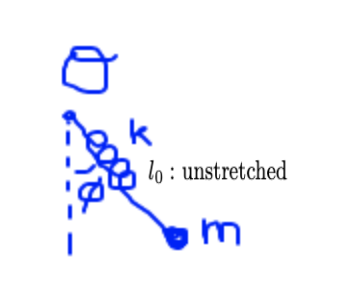
\includegraphics[width=0.3\textwidth]{hw2_fig1.png}
    \caption{An illustration of the pendulum and spring configuration.}
\end{figure}

\hrule
         \ \ \ 

\subsection*{(a) Write down the Lagrangian for the pendulum, using as generalized coordinates the usual angle $\phi$ and the length $r$ of the spring.}
To find the Lagrangian, $\mathcal{L}$, we must first find the kinetic and potential energies. 

$$\mathcal{L} = T - U$$
As the spring is massless, it is clear the only kinetic energy of the system is the kinetic energy of the mass. We will use polar coordinates around the fixed pivot location as this is convenient. We will define $\phi$ to be zero when the mass is directly below the fixed pivot along the dotted line shown in Figure 1. We will also define $\phi$ to be positive in the counterclockwise direction around the $\phi=0$ dotted line. In polar coordinates, the velocity of the mass is of the form:
    \begin{align*}
    v^2 &= r^2 + (r\dot{\phi})^2 \\
    v^2 &= r^2 + r^2\dot{\phi}^2
    \end{align*}
Therefore we have the total kinetic energy T, 
$$T = \frac{1}{2}m(r^2 + r^2\dot{\phi}^2)$$
This system has two forms of potential energy, gravitational potential energy and elastic potential energy from the spring.

$$U = U_G + U_S$$
We can set the gravitational potential energy to be zero at a height of the pivot. Therefore,


$$U_G = -mgr(cos(\phi))$$
It is clear that the elastic potential energy is of the form:

$$U_S = \frac{1}{2}k(r-l_0)^2$$
$$U = -mgr(cos(\phi)) + \frac{1}{2}k(r-l_0)^2$$
Putting this all together we have the Lagrangian. 

\begin{align*}
\mathcal{L} &= T - U\\
\mathcal{L} &= \frac{1}{2}m(r^2 + r^2\dot{\phi}^2) - \left( mgr(cos(\phi)) + \frac{1}{2}k(r-l_0)^2 \right) 
\end{align*}
$$\boxed{\mathcal{L} = \frac{1}{2}m(r^2 + r^2\dot{\phi}^2) +mgr(cos(\phi)) - \frac{1}{2}k(r-l_0)^2}$$


\subsection*{(b) Find the two Lagrange equations of the system and interpret them in terms of Newton's Second Law.}

We will find the equations of motion using, as usual, Lagrange's equations. We can first do this for our generalized coordinate $\phi$:
\begin{align*}
\pdv{\mathcal{L}}{\phi} &= \odv{}{t} \pdv{\mathcal{L}}{\dot{\phi}}\\
\pdv{\mathcal{L}}{\phi} &= -mgr(sin(\phi))\\
\odv{}{t} \pdv{\mathcal{L}}{\dot{\phi}} &= \odv{}{t}(mr^2\dot{\phi}) = 2mr\dot{r}\dot{\phi} + mr^2\ddot{\phi}      \\
\end{align*}
Putting this together we have the equation of motion for the mass in the $\phi$ direction. 
$$2mr\dot{r}\dot{\phi} + mr^2\ddot{\phi} = -mgr(sin(\phi))$$
$$\boxed{m(2\dot{r}\dot{\phi} + r\ddot{\phi}) = -mg(sin(\phi))}$$
This equation makes sense and we can interpret it in terms of Newton's Second Law. In polar coordinates, acceleration in the $\phi$ direction is $2\dot{r}\dot{\phi} + r\ddot{\phi}$. It is clear that $-mg(sin(\phi))$ is the component of the force of gravity in the $\phi$ direction. As the spring force only acts in the radial direction we do not get any component of it in out equation of motion. Therefore, this Lagrangian equation gives us Newton's Second Law in the $\phi$ direction. 
$$m\underbrace{(2\dot{r}\dot{\phi} + r\ddot{\phi})}_{a_{\phi}} = \underbrace{-mg(sin(\phi))}_{F_{G,\phi}}$$
We can now find the equation of motion in the radial equation with out other Lagrange equation. 
\begin{align*}
\pdv{\mathcal{L}}{r} &= \odv{}{t} \pdv{\mathcal{L}}{\dot{r}}\\
\pdv{\mathcal{L}}{r} &= m\dot{\phi}^2r + mg(cos(\phi))- k(r-l_0)\\
\odv{}{t} \pdv{\mathcal{L}}{\dot{\phi}} &= \odv{}{t}(m\dot{r}) = m\ddot{r}      \\
\end{align*}
Putting this together we have the equation of motion for the mass in the radial direction. 
$$m\ddot{r} = m\dot{\phi}^2r +  mg(cos(\phi))- k(r-l_0) $$
$$\boxed{m (\ddot{r} - \dot{\phi}^2r) =  mg(cos(\phi))- k(r-l_0)}$$
This equation makes sense and we can once again interpret it in terms of Newton's Second Law. In polar coordinates, the radial acceleration is $\ddot{r} - \dot{\phi}^2r$. It is clear that $mg(cos(\phi))$ is the component of the force of gravity acting in the radial direction. It is also clear that $- k(r-l_0)$ is the force of the spring. Therefore, this Lagrange equation gives us Newtons Second Law in the radial direction.
$$m\underbrace{(\ddot{r} - \dot{\phi}^2r)}_{a_r} = \underbrace{mg(cos(\phi))}_{F_{G,r}} \underbrace{-k(r-l_0)}_{F_S}$$

\subsection*{(c) The equations of part (b) cannot be solved analytically in general. However, they can be solved for small oscillations. Do this and describe the motion.}

Small oscillations in the radial direction will be defined as $\epsilon$. We can define $l$ to be the equilibrium length of the spring. Therefore, it is clear that $r = l+ \epsilon$. As the oscillations are small, the equilibrium length, $l$, is the length where the gravitational force is equal to the spring force. 
\begin{align*}
F_G &= F_S\\
mg &= k(l-l_0)\\
l &= \frac{mg}{k} - l_0
\end{align*}
We will use this later. Since $r= l+ \epsilon$, $\dot{r} = \dot{\epsilon}$ and $\ddot{r} = \ddot{\epsilon}$. Also, using only first order terms since the oscillations are small, $sin(\phi) \approx \phi$ and  $cos(\phi) \approx 1$. Substituting this into our equations of motion we get:
$$m (\ddot{\epsilon} - \dot{\phi}^2(l+ \epsilon)) =  mg- k((l+ \epsilon)-l_0)$$

$$m(2\dot{\epsilon}\dot{\phi} + (l + \epsilon)\ddot{\phi}) = -mg\phi$$
For these small oscillations, since $\phi$ and $\epsilon$ are so small we can drop all the powers of $\phi$ and $\epsilon$ (as well as their derivatives and products) that are higher than first order. 
$$m\ddot{\epsilon} =  mg- k(l+ \epsilon-l_0)$$
$$m(l + \epsilon)\ddot{\phi} = -mg\phi$$
In addition, since the oscillations are small, $l + \epsilon \approx l$. 
$$m\ddot{\epsilon} =  mg- k(l+ \epsilon-l_0)$$
$$ml\ddot{\phi} = -mg\phi$$
Looking at the ladder equation, the equation of motion in the radial direction, we can simply it by substituting in our calculated equilibrium length, $l$. 
\begin{align*}
    m\ddot{\epsilon} &=  mg- k(\frac{mg}{k} - l_0+ \epsilon-l_0)\\
    m\ddot{\epsilon} &=  mg- k(\frac{mg}{k} + \epsilon)\\
    m\ddot{\epsilon} &=  mg- k\frac{mg}{k} - k\epsilon\\
    m\ddot{\epsilon} &=  mg- mg - k\epsilon\\
    m\ddot{\epsilon} &=   - k\epsilon\\
    \ddot{\epsilon} &=   - \frac{k}{m}\epsilon\\
\end{align*}
It is clear that this is simple harmonic motion. This has the solution:
$$\epsilon = C_1 sin(\sqrt{\frac{k}{m}}t + C_2)$$
Substituting this into $r = l + \epsilon$, we find the equation of motion of the mass for small oscillations in the radial direction. 
$$r = l + C_1 sin(\sqrt{\frac{k}{m}}t + C_2)$$
$$\boxed{r = \frac{mg}{k} - l_0+ C_1 sin(\sqrt{\frac{k}{m}}t + C_2)}$$
where $C_1$ and $C_2$ are constants that can be determined by initial condition. $\newline$
Solving at the equation of motion in the $\phi$ direction:
\begin{align*}
    ml\ddot{\phi} &= -mg\phi \\
    \ddot{\phi} &= -\frac{g}{l}\phi \\
\end{align*}
It is clear that this is simple harmonic motion. This has the solution:
$$\boxed{\phi = C_3 sin(\sqrt{\frac{g}{l}}t + C_4)}$$
where $C_3$ and $C_4$ are constants that can be determined by initial condition. $\newline$
This assumption greatly simplified and uncoupled the equations. The result is simple harmonic motion due to the spring in the radial direction and simple harmonic motion due to the pendulum in the $\phi$ direction. 





\end{document}